\section{Resonances}


%----------------------------------------
%
%----------------------------------------

\begin{figure}[H]
    \centering
    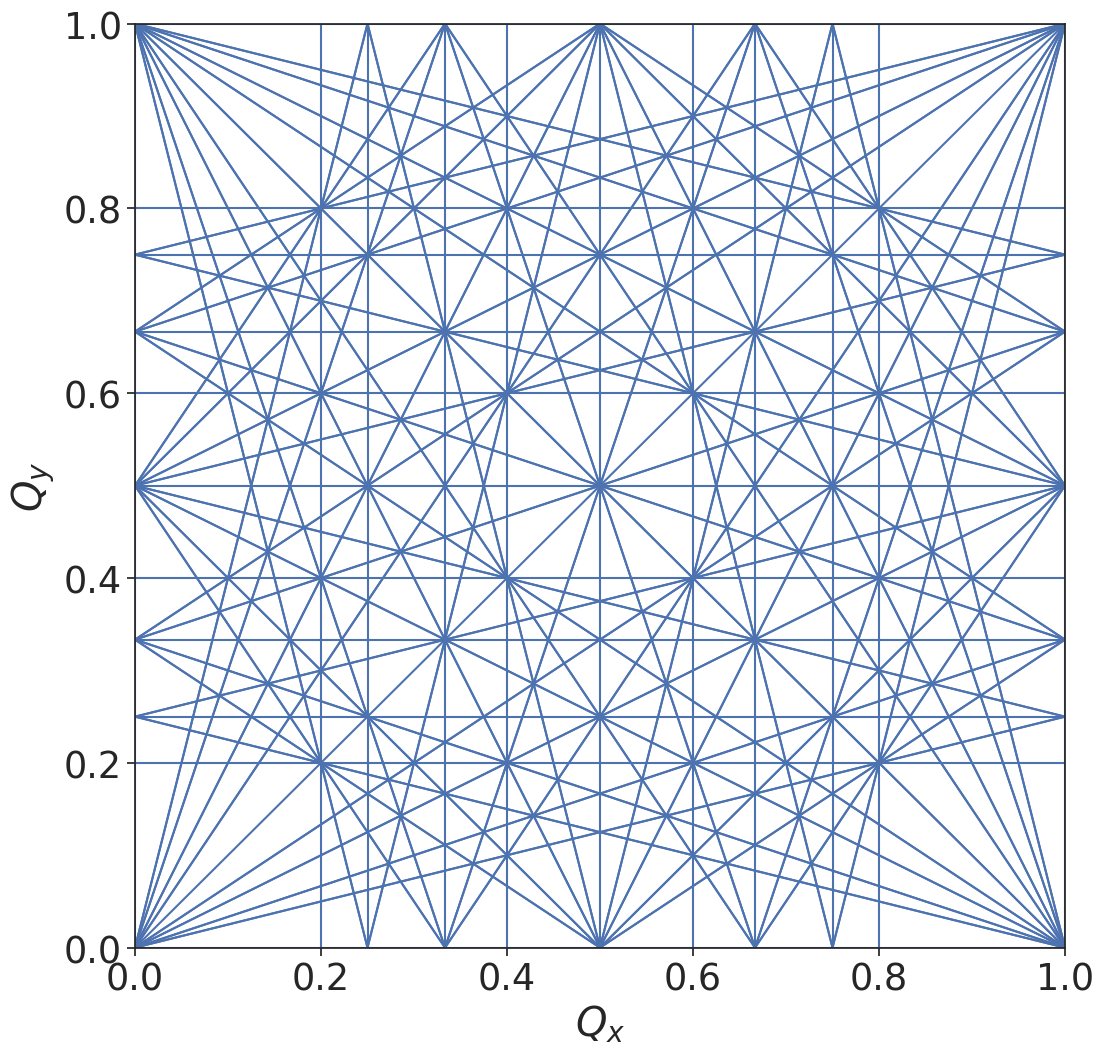
\includegraphics[width=0.7\textwidth]{images/resonance_diagaram_n5.png}
    \caption{Tune diagram with resonances lines excited by multipoles up to decapole ($n \leq 5$).
             The working point of the machine is chosen in an area where few lines are present.}
    \label{fig:resonances:diagram_n5}
\end{figure}


\begin{figure}[H]
    \centering
    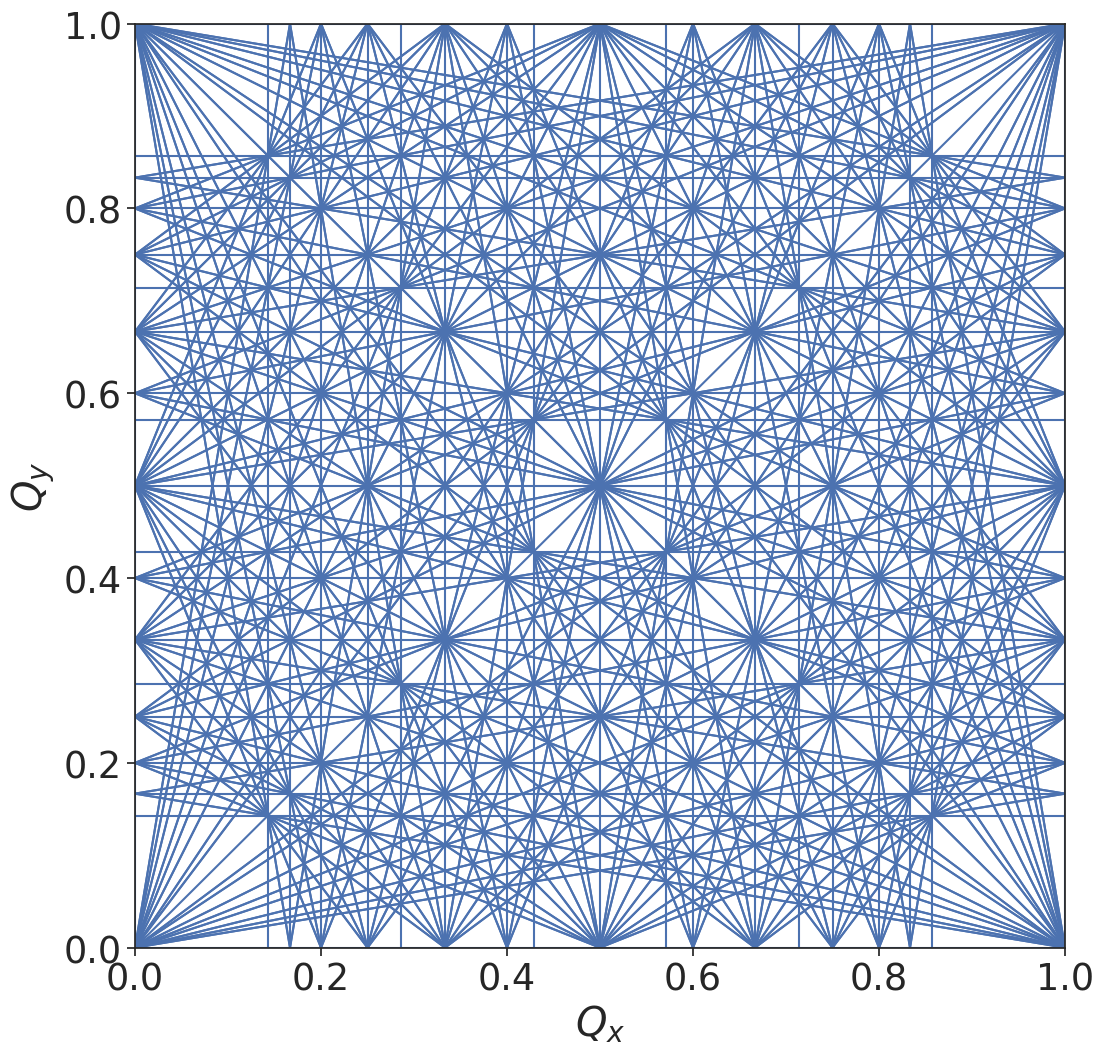
\includegraphics[width=0.7\textwidth]{images/resonance_diagaram_n7.png}
    \caption{Tune diagram with resonances lines excited by multipoles up to decatetrapole 
             ($n \leq 7$). When considering higher orders, it becomes apparent that the beam will
             hit several resonances.}
    \label{fig:resonances:diagram_n7}
\end{figure}